\chapter{Examples}\label{sec:ex}
This is a collection of validated (with the software \neweulm \cite{kurz_neweul_2010}) examples: \\
\begin{tabular}{|l|l|}
\hline
Examples/RA3Link/ & 3-link robot arm (\secref{sec:3link}) \\ \hline
Examples/RA3LinkPrismatic/ & 3-link robot arm with prismatic joint (\secref{sec:3linkPris}) \\ \hline
Examples/QuadrupedFreeFloat/ & free floating quadruped (\secref{sec:quadruped}) \\ \hline
\end{tabular}

%%%%%%%%%%%%%%%%%%%%%%%%%%%%%%%%%%%%%%%%%%%%%%%%%%%%%%%%%%%%%%%%%%%%%%%%%%%%%%%%%%%%%%%%%%
\section{3-link Robot Arm} \label{sec:3link}
\begin{figure} [H]
	\centering
		\subfigure[3-link arm]{\includegraphics[width=0.4\textwidth]{../RobotArmExample/robotArm3link_asm.pdf}}\qquad
		\subfigure[Description of the second body]{\includegraphics[width=0.5\textwidth]{../RobotArmExample/robotArm3link_plotBodies}}	
	\caption{3-link robot arm with three revolute joints ($\mathbf{z},\mathbf{x},\mathbf{y}$).}
	\label{fig:3D_PR}
\end{figure}

\lstinputlisting{../../examples/RA3Link/genEoM.m}

%%%%%%%%%%%%%%%%%%%%%%%%%%%%%%%%%%%%%%%%%%%%%%%%%%%%%%%%%%%%%%%%%%%%%%%%%%%%%%%%%%%%%%%%%%%%%
\clearpage
\section{3-link Robot Arm with Prismatic Joint} \label{sec:3linkPris}
\begin{figure}[H]
	\centering
		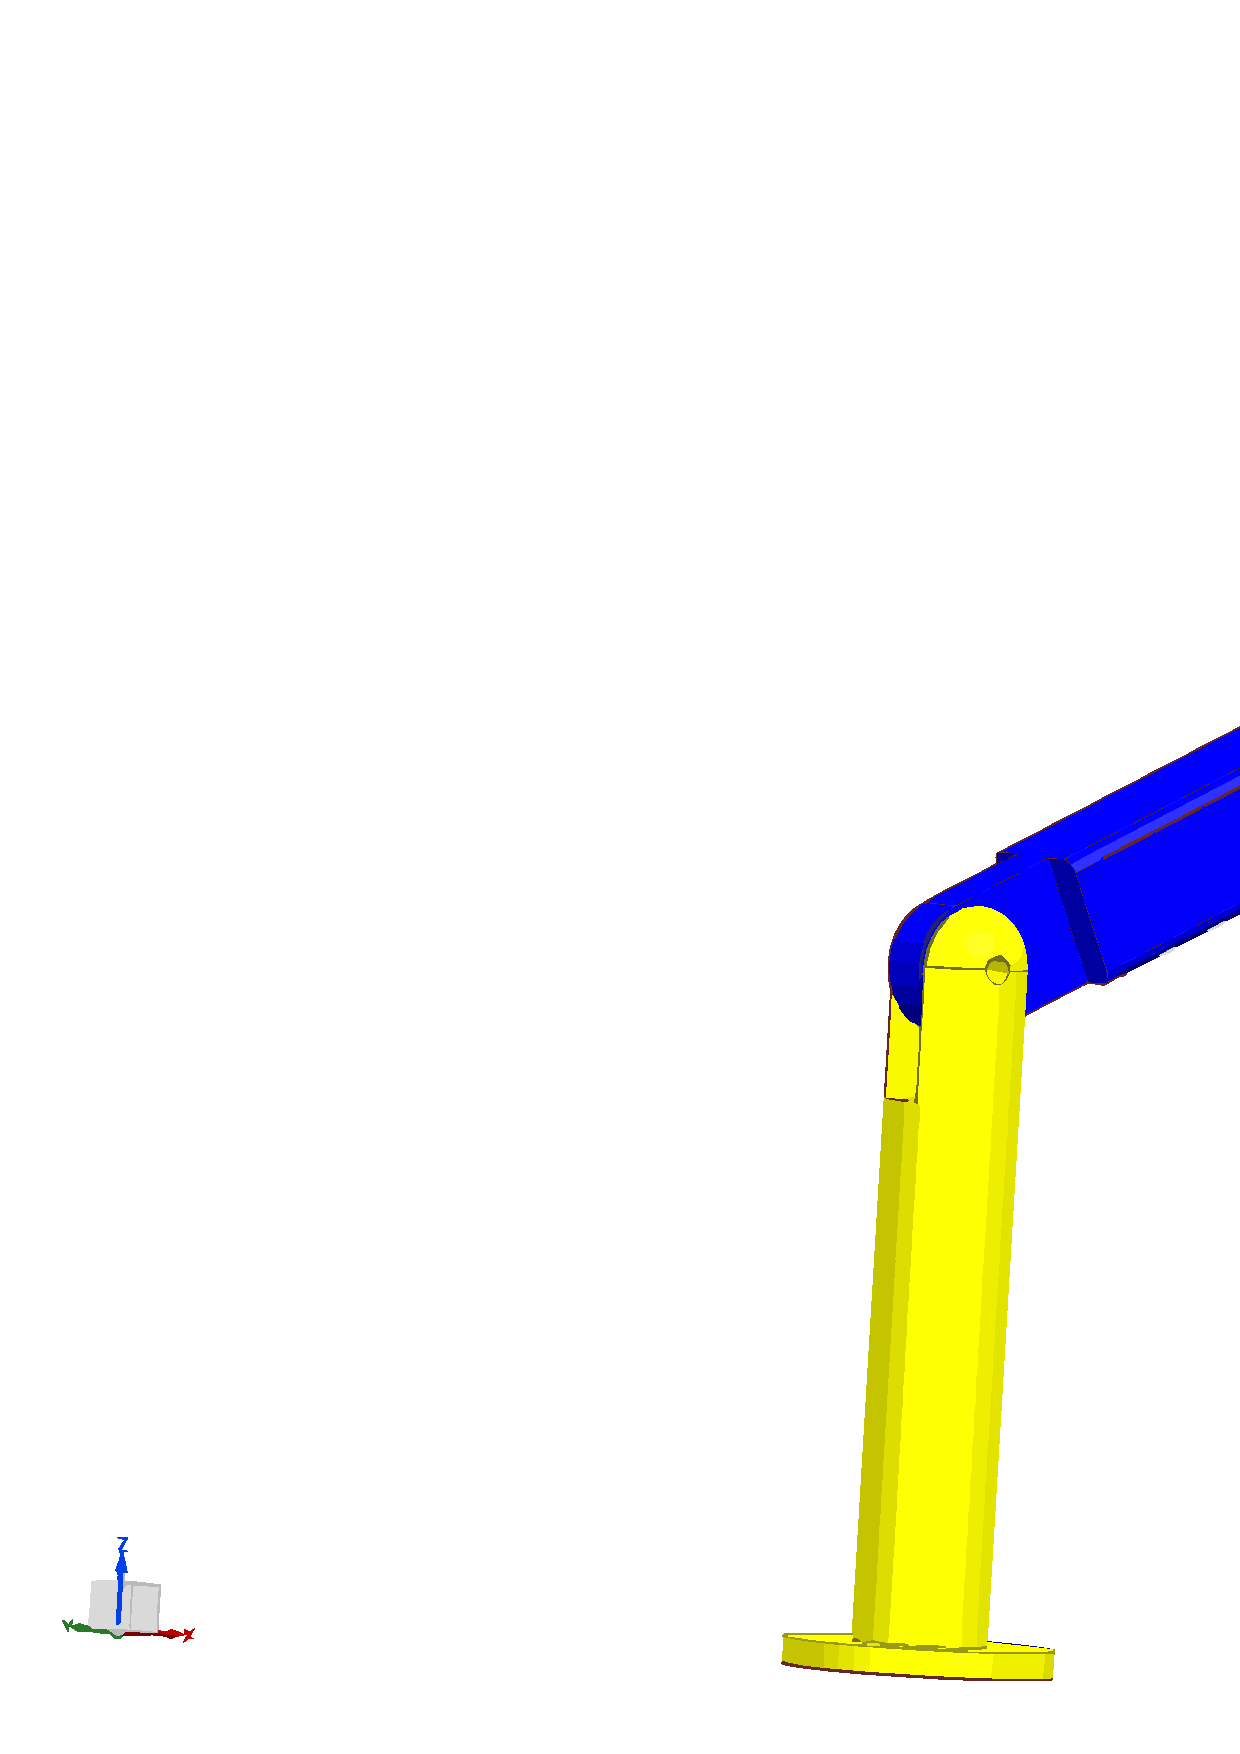
\includegraphics[width=0.50\textwidth]{../RobotArmExample/robotArm_asm.pdf}
	\caption{3-link robot arm with two revolute joints ($\mathbf{z},\mathbf{y}$) and one prismatic joint ($\mathbf{x}$).}
	\label{fig:robotArm_asm}
\end{figure}


\lstinputlisting{../../examples/RA3LinkPrismatic/genEoM.m}


%%%%%%%%%%%%%%%%%%%%%%%%%%%%%%%%%%%%%%%%%%%%%%%%%%%%%%%%%%%%%%%%%%%%%%%%%%%%%%%%%%%%%%%%%%%%%
\clearpage


\section{Quadruped Robot Starl\textit{ETH}}\label{sec:quadruped}
For detailed information about our quadruped Starl\textit{ETH} please consult our homepage\footnote{leggedrobotics.ethz.ch}.  Here is a brief outline: each leg has 3 degrees of freedom (x-rotation for hip abduction/adduction, followed by y-rotation for hip flexion/extension as well as y-rotation for knee flexion/extension) and is connected to a free floating main body.
\\
This model shows also how to model a free floating body as well as ground contact.  Adding dummy-bodies as feet allow to directly get the support Jacobians needed for modeling the hard ground contact (impact as well as contact constraints).
\begin{figure} [H]
	\centering
		\subfigure[]{\includegraphics[width=0.5\textwidth]{pics/3D_PR.pdf}}\qquad
		\subfigure[]{\includegraphics[width=0.4\textwidth]{pics/starleth_frames.png}}	
	\caption{Free floating quadruped Starl\textit{ETH} with a total of 18 DoF.}
	\label{fig:quadruped}
\end{figure}



\lstinputlisting{../../examples/QuadrupedFreeFloat/genEoM.m}


%%%%%%%%%%%%%%%%%%%%%%%%%%%%%%%%%%%%%%%%%%%%%%%%%%%%%%%%%%%%%%%%%%%%%%%%%%%%%%%%%%%%%%%%%%%%%
\clearpage
\section{Generating Code} \label{sec:code}
There are different possibilities to generate code that can be embedded in simulations or controllers:
\begin{itemize}
\item .m function
\item compiled mex functions
\item C-code to embed
\end{itemize}

The matlab script \emph{createFunctionFiles.m} gives you some example code.

\subsection{Generating Matlab Functions and Mex Functions}
% change here the line numbers
%\lstinputlisting[firstline=40, lastline=52]{../../examples/GeneratingCode/createFunctionFiles.m}.
The Symbolic Toolbox of Matlab provides the function \emph{matlabFunction} to generate a matlab function from a symbolic matrix in a m-file:

\begin{lstlisting}
% generate a matlab function
matlabFunction(sys.MpNE,'file','matlabFunc/Mfunc','vars',[sys.q;sys.param]);
matlabFunction(sys.bpNE,'file','matlabFunc/bfunc','vars',[sys.q;sys.dq;sys.param]);
matlabFunction(sys.gpNE,'file','matlabFunc/gfunc','vars',[sys.q;sys.param]);
\end{lstlisting}

The generated files can be used to compile \emph{mex-files} as follows:

\begin{lstlisting}
% compile this matlab function to a mex function
emlc -o mexFunc/Mfunc_mex matlabFunc/Mfunc.m
emlc -o mexFunc/bfunc_mex matlabFunc/bfunc.m
emlc -o mexFunc/gfunc_mex matlabFunc/gfunc.m
\end{lstlisting}

Note: The mex-functions are executed much faster than the matlab-functions for systems with a lot of degrees of freedom.

\subsection{Generating C-Code}
The Symbolic Toolbox of Matlab comes along with the function \emph{ccode} that generates C-code from a symbolic matrix.
The function \emph{ccode} is able to write optimized C-Code in a file. 
Note that the function can also print the code in the command window of Matlab, but that code is not optimized. 


The function \emph{ccode} makes extensive use of auxiliary variables that need to be defined, e.g. as 'const double'.
The following function adds the definitions and re-names the array name:
\lstinputlisting[firstline=1, lastline=13]{../../examples/GeneratingCode/genCCodeMatrix.m}

The function creates a temporary file that could be included somewhere in your code, and outputs the C-code in string.


The Matlab function \emph{genCCodeMatrix} does not add a definition of the array, e.g. 
\begin{lstlisting}
 double MpNE[3][3];
\end{lstlisting}
because the definition might be in another location of your code, e.g. in a class as a member variable.
Moreover, the array needs to be initialized with zero values, because the function \emph{ccode} omits array entries that are zero.


The following Matlab function is an example for generating C-code:
\lstinputlisting[firstline=1, lastline=13]{../../examples/GeneratingCode/genCCodeExampleFile.m}

It creates a simple application that computes the components of the EoM and prints them to the command line.


